\documentclass[a4paper]{article}
\usepackage{graphicx}
\usepackage{amsfonts}
\usepackage[ruled,vlined]{algorithm2e}
\usepackage[a4paper, total={6in, 10in}]{geometry}
\setlength{\belowcaptionskip}{-10pt}
\graphicspath{ {./images/} }
\title{Unsupervised Data Augmentation Experiments}
\author{Michael Morris}

\begin{document}
\maketitle
\section{Semi Supervised Learning}
Semi supervised learning is a method of training machine learning models which leverages unlabelled data. This reduces the labelling cost of an expert labeller and means that datasets with large amounts of unlabelled data can be used. Historically this has been done by generating a decision boundary based on the positions of unlabelled data in relation to labelled data. 

\begin{figure}[h]
  \begin{center}
    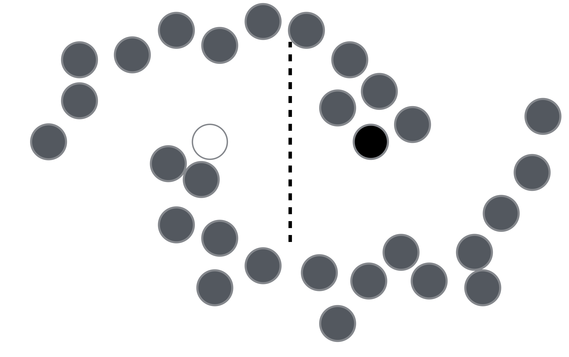
\includegraphics[width=.4\textwidth]{SSL}
    \caption{Decision boundary with unsupervised examples}
  \end{center}
\end{figure}
The unlabelled datapoints can be categorised correctly by their spatial relation to the two labelled samples. The methods to do this are based on the following assumptions:
\begin{itemize}
  \item Points which are close together are likely to be in the same class 
  \item The data tends to form distinct clusters
  \item The data can be expressed in fewer dimensions than its inputs.
\end{itemize}
These lead to pseudo labelling where the model is updated as if these labels are correct. 

\section{Unsupervised Data Augmentation}
Unsupervised Data Augmentation (UDA) is a method of leveraging unlabelled data based on state of the art data augmentation policies. In UDA unlabelled data is augmented: $\hat{x}=q(x,\epsilon)$ and the divergence in outputs between the original and augmented data is minimised for consistency training. This follows the assumption that the original and augmented samples have the same class, and by learning distinguishing features the distance between the labelled and unlabelled data will be minimised. The loss function for the labelled data is categorical cross entropy. For the unlabelled data is the Kullback-Leibler divergence between the original and augmented data. The unsupervised loss is weighted by a variable $\lambda$ giving the full objective function where $U$ and $L$ represent unlabelled and labelled data respectively:
\begin{equation}
\min_{\theta} \mathcal{J}(\theta) =\mathbb{E}_{x,y^* \in L}[-\log p_\theta (y^* | x)]+\lambda\mathbb{E}_{x \in U}\mathbb{E}_{\hat{x}\sim q(\hat{x} \mid x)}[\mathcal{D}_{KL}(p_{\tilde{\theta}}(y \mid x) \parallel p_\theta (y \mid \hat{x})) ]
\end{equation}

Where the KL divergence is:
\begin{equation}
\mathcal{D}_{KL}(P \parallel Q) = \sum_{x \in X} P_{(x)} \log \left(\frac{P_{(x)}}{Q_{(x)}}\right)
\end{equation}

The training objective is illustrated in Figure \ref{fig:objective} and leads to the pseudocode in Algorithm \ref{alg:UDAAlg}
\begin{figure}[!ht]
  \begin{center}
    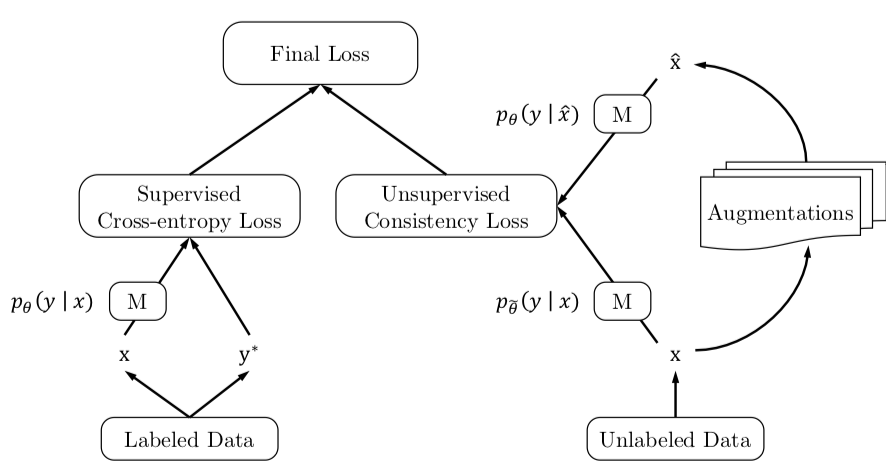
\includegraphics[width=.7\textwidth]{training_objective}
    \caption{Training objective for UDA}
    \label{fig:objective}
  \end{center}
\end{figure}
\subsection{Training Signal Annealing}
A common problem when running UDA is overfitting to the few labelled training samples. To combat this a technique Training Signal Annealing (TSA) is used which gradually releases training signals from labelled data into the loss function. When the model predicts the correct class of a training example with a confidence above a set threshold it is removed from the loss function. The threshold is increased during training from a worst case of $\frac{1}{K}$ to $1$. Where $K$ is the number of classes in the dataset. For the $t^th$ iteration out of $T$ total iterations the threshold $n_t$ is $\alpha_{t} * (1-\frac{1}{K})+\frac{1}{K}$. $\alpha_t$ is either: logarithmic $1-\exp(\frac{t}{T} * 5)$, linear $t/T$, or exponential: $\exp(({t}{T}-1)*5)$. The fewer labelled training samples you have the more slowly the training samples should be released. 
\begin{figure}[!ht]
  \begin{center}
    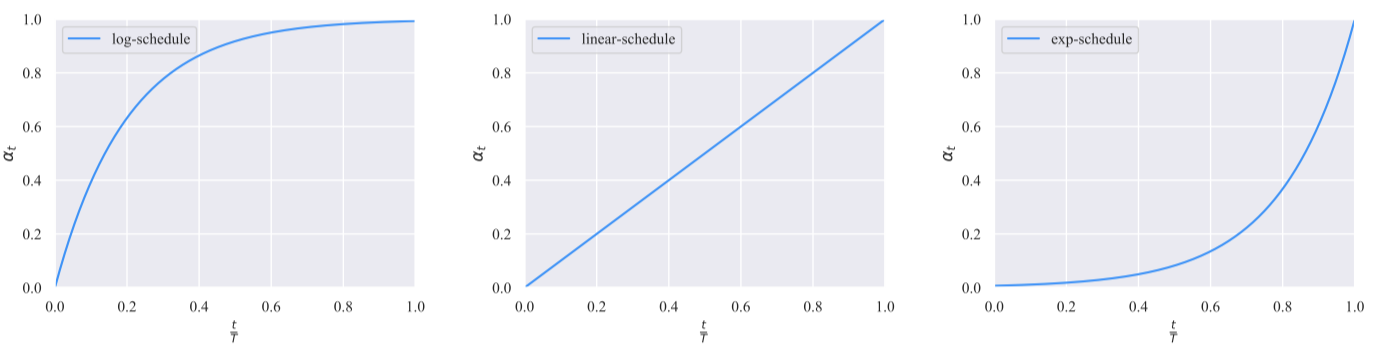
\includegraphics[width=0.9\textwidth]{TSA}
    \caption{TSA Schedules}
    \label{fig:objective}
  \end{center}
\end{figure}
\begin{algorithm}[!ht]
\SetAlgoLined
duplicate data so equal number of potential batches in labelled and unlabelled sets\;
shuffle and split into batches\;
 \For{epochs}{
 	\For{batches}{
		\If{labelled batch}{
			calculate $p_\theta (y^* | x)$\;
   			$Lloss = \mathbb{E}_{x,y^* \in L}[-\log p_\theta (y^* | x)]$\;
			Apply training signal annealing
		}
		\If {unlabelled batch}{
			create $\hat{x}$ by augmenting $x$\;
			$Uloss = \lambda\mathbb{E}_{x \in U}\mathbb{E}_{\hat{x}\sim q(\hat{x} \mid x)}[\mathcal{D}_{KL}(p_{\tilde{\theta}}(y \mid x) 	\parallel p_\theta (y \mid \hat{x})) ]$\;
		}
		minimise $Uloss+Lloss$\;
 	}
	calculate accuracy from labelled validation set\;
 }
\caption{UDA Algorithm}
\label{alg:UDAAlg}
\end{algorithm}

\subsection{Experiments}
Experiments were carried out on the MNIST and CIFAR10 datasets, a convolutional neural network with 3 convolutional layers, 1 hidden layer and a softmax output layer was used for both, the only difference being the shape of the inputs (MNIST: 28,28,1,   CIFAR10: 32,32,3). 
\subsubsection{MNIST}
The MNIST dataset was split into 42000 training samples, and 18000 testing samples, within the training set 10\% was reserved for cross validation. With a fully supervised learning using cross entropy as the loss function an error rate of 0.458\% was achieved. 

\subsection{CIFAR10}
The CIFAR10 dataset was split into 10000 test samples and 50000 training samples where 4000 are labelled and 46000 unlabelled to replicate the experiments in the original paper. 

\end{document}